\chapter{CITATIONS AND REFERENCES}

\section{Citations}
  Cite your references using BibTeX.
  You can cite individual references one at a time \cite{hawking1975particle}, \cite{einstein1915general}, \cite{turing1936computable}.
  You can also cite multiple references at once \cite{hawking1975particle,einstein1915general,turing1936computable}.

\section{References to Figures, Tables, Equations, etc.}
  When referring to numbered entities in the text, never hardcode figure/table/equation numbers.
  Use \verb|\ref| to refer to them, so they update automatically if you add or remove figures.
  Make sure to put \verb|\label| after \verb|\caption| for tables and figures, and after the equation for equations, so that the numbering works correctly.

  For example, see Table~\ref{tab:references}, Figure~\ref{fig:moon-crust}, Figure~\ref{fig:saturn-hexagon}, (\ref{eq:pythagorean-theorem}), and (\ref{eq:quadratic-formula}).

  \begin{table}[h]
    \caption{Example references from the bibliography.}\vspace{0.5em}
    \label{tab:references}
    \centering
    \begin{tabular}{|c|L{3in}|}
      \hline
      \textbf{Reference} & \textbf{Description} \\
      \hline
      \texttt{hawking1975particle} & Hawking's seminal paper on black hole radiation. \\
      \hline
      \texttt{einstein1915general} & Einstein's paper on the general theory of relativity. \\
      \hline
      \texttt{turing1936computable} & Turing's paper on computable numbers and the Turing machine. \\
      \hline
    \end{tabular}
  \end{table}

  \begin{figure}[htbp]
    \centering
    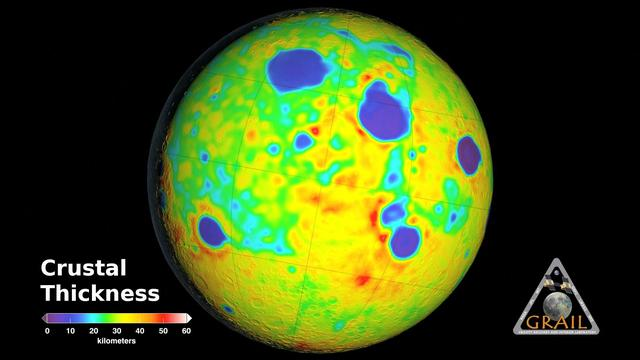
\includegraphics[width=0.5\textwidth]{../img/moon_crust.jpg}
    \caption{Map of the moon's crust thickness.}
    \label{fig:moon-crust}
  \end{figure}

  \begin{figure}[htbp]
    \centering
    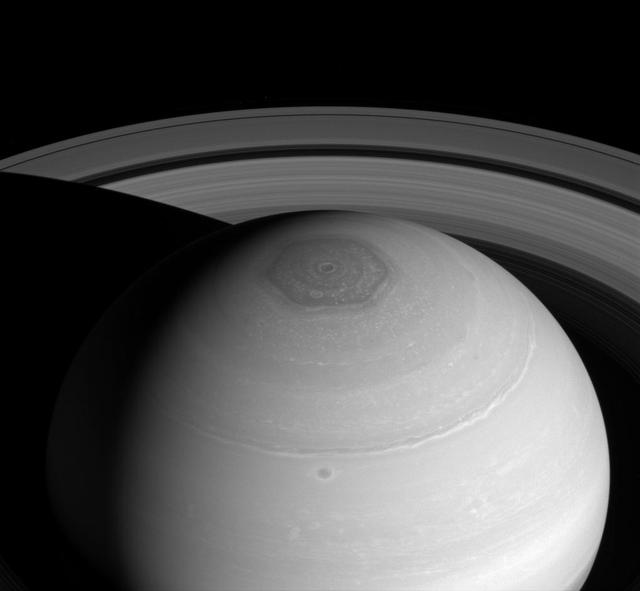
\includegraphics[width=0.5\textwidth]{../img/saturn_hexagon.jpg}
    \caption{Saturn's weird North pole hexagon.}
    \label{fig:saturn-hexagon}
  \end{figure}

    \begin{equation}
    a^2 + b^2 = c^2
    \label{eq:pythagorean-theorem}
  \end{equation}

  \begin{equation}
    x = \dfrac{-b \pm \sqrt{b^2 - 4ac}}{2a}
    \label{eq:quadratic-formula}
  \end{equation}